\begin{frame}{Homogeneous Coordinates}
  \begin{columns}[T,onlytextwidth]
    \column{0.57\textwidth}
      \begin{itemize}\footnotesize\itemsep0.3em
        \item \textbf{Homogeneous coordinates:} write the pixel $(u,v)$ as the 3-vector $(wu,\,wv,\,w)^\top$ for any $w\neq0$. All of them are the same point, $\tilde{\mathbf{x}}=(u,v,1)^\top\sim(wu,wv,w)^\top$, where $\sim$ means equal up to a nonzero scale.
        \item Back to pixels: divide by the last entry, $(x_1,x_2,x_3)^\top\mapsto(x_1/x_3,\;x_2/x_3)$. Example: $(6,4,2)^\top\sim(3,2,1)^\top$ is the pixel $(3,2)$.
        \item \textbf{Points at infinity} have $w=0$: $(1,2,0)^\top$ is the direction $(1,2)$, the point where all lines with that direction meet.
        \item \textbf{Lines} are 3-vectors too: $\mathbf{l}=(a,b,c)^\top$ is the line $au+bv+c=0$, so $\tilde{\mathbf{x}}$ lies on it exactly when $\mathbf{l}^\top\tilde{\mathbf{x}}=0$. Two lines meet at $\mathbf{l}_1\times\mathbf{l}_2$: the parallel lines $u=1$ and $u=2$, i.e.\ $(1,0,-1)^\top$ and $(1,0,-2)^\top$, meet at $(0,1,0)^\top$, the point at infinity in the $v$ direction.
        \item \textbf{Why:} perspective division becomes a matrix product (next slide), and a rotation plus a translation of a 3D point, written as the 4-vector $(X,Y,Z,1)^\top$, becomes a single $4\times4$ matrix.
      \end{itemize}
    \column{0.41\textwidth}
      \centering
      \vspace{0.3em}
      \begin{tikzpicture}[font=\sffamily\scriptsize, >=latex, x={(0.45cm,0.32cm)}, y={(0cm,1.0cm)}, z={(1.5cm,0cm)}]
        \draw[->, black!60] (0,0,0) -- (0,0,2.75) node[right, black] {$w$};
        \draw[->, black!60] (0,0,0) -- (0,1.25,0) node[above, black] {$v$};
        \draw[->, black!60] (0,0,0) -- (1.25,0,0) node[above right=-1pt, black] {$u$};
        \filldraw[draw=blue!60!black, fill=blue!10, fill opacity=0.8] (-1,-0.9,1) -- (1,-0.9,1) -- (1,1.1,1) -- (-1,1.1,1) -- cycle;
        \node[blue!50!black, anchor=north west] at (1,-0.9,1) {plane $w=1$};
        \draw[thick, red!70!black, ->] (0,0,0) -- (1.15,1.265,2.3);
        \fill (0,0,0) circle (1.5pt) node[below] {origin};
        \fill[red!70!black] (0.5,0.55,1) circle (1.6pt) node[above left=1pt and -1pt, black] {$(u,v,1)$};
        \fill[red!70!black] (1,1.1,2) circle (1.6pt) node[above left=1pt and -1pt, black] {$(2u,2v,2)$};
      \end{tikzpicture}\\[0.4em]
      {\scriptsize Every homogeneous vector is a ray through the origin; the pixel is where that ray meets the plane $w=1$. After Hartley and Zisserman (2004), Ch.~2.\par}
  \end{columns}
\end{frame}

\begin{frame}{The Pinhole Camera Model}
  \begin{columns}[T,onlytextwidth]
    \column{0.50\textwidth}
      \begin{itemize}\footnotesize\itemsep0.3em
        \item \textbf{Pinhole model:} every ray from a scene point $\mathbf{X}=(X,Y,Z)^\top$ passes through the optical centre $C$ and meets the image plane at distance $f$ (the focal length) behind $C$, upside down. A virtual plane at $f$ in front of $C$ gives the same image unflipped; later figures use it.
        \item Camera coordinates: origin at $C$, $Z$ along the optical axis (the line through $C$ perpendicular to the image plane), $X$ and $Y$ parallel to the image axes. Similar triangles give
        \[ x = f\,\frac{X}{Z},\qquad y = f\,\frac{Y}{Z}\qquad (Z>0), \]
        with $(x,y)$ in the units of $f$, e.g.\ millimetres.
        \item In homogeneous coordinates the division becomes the scale, with $\tilde{\mathbf{X}}=(X,Y,Z,1)^\top$:
        \[ \begin{pmatrix} x\\ y\\ 1\end{pmatrix} \sim \begin{pmatrix} fX\\ fY\\ Z\end{pmatrix} = \begin{bmatrix} f&0&0&0\\ 0&f&0&0\\ 0&0&1&0\end{bmatrix}\tilde{\mathbf{X}}. \]
      \end{itemize}
    \column{0.48\textwidth}
      \centering
      \vspace{0.6em}
      \begin{tikzpicture}[font=\sffamily\scriptsize, >=latex, scale=0.86, every node/.style={transform shape}]
        \coordinate (C) at (0,0);
        \coordinate (X) at (4.5,2.0);
        \coordinate (xv) at ($(C)!0.266667!(X)$);
        \coordinate (xr) at ($(C)!-0.266667!(X)$);
        \fill[green!14] (C) -- (4.5,0) -- (X) -- cycle;
        \fill[orange!30] (C) -- (1.2,0) -- (xv) -- cycle;
        \draw[dashed, gray] (-1.7,0) -- (5.3,0) node[right, black] {$Z$};
        \draw[thick, blue!60!black] (1.2,-0.9) -- (1.2,1.3) node[above, align=center] {virtual\\image plane};
        \draw[thick, black!45] (-1.2,-1.3) -- (-1.2,0.9) node[above, align=center, text=black!70] {real image\\(inverted)};
        \draw[thick, red!70!black] (xr) -- (X);
        \fill (C) circle (1.6pt) node[above left] {$C$};
        \fill[red!70!black] (X) circle (1.6pt) node[above] {$\mathbf{X}=(X,Y,Z)$};
        \fill[red!70!black] (xv) circle (1.5pt);
        \fill[black!55] (xr) circle (1.5pt);
        \draw[|<->|] (4.85,0) -- (4.85,2.0) node[midway, right] {$Y$};
        \draw[|<->|] (1.45,0) -- (1.45,0.533333) node[midway, right] {$y$};
        \draw[|<->|] (0,-0.45) -- (1.2,-0.45) node[midway, below] {$f$};
        \draw[|<->|] (0,-1.05) -- (4.5,-1.05) node[midway, below] {$Z$};
      \end{tikzpicture}\\[0.4em]
      {\scriptsize Side view. The ray from $\mathbf{X}$ through $C$ meets the virtual plane at $y=fY/Z$ and the real image at $-fY/Z$; the two shaded triangles are similar. The depth $Z$ is divided out, so a single pixel cannot return it. Camera model after Hartley and Zisserman (2004), Ch.~6.\par}
  \end{columns}
\end{frame}

\begin{frame}{Intrinsics: From Image Plane to Pixels}
  \begin{columns}[T,onlytextwidth]
    \column{0.55\textwidth}
      \begin{itemize}\footnotesize\itemsep0.3em
        \item Pixels are not millimetres: each sensor pixel has a pitch (size) $\rho_x\times\rho_y$, and pixel $(0,0)$ sits at the top-left corner, away from the optical axis.
        \item \textbf{Intrinsics $K$:} with the depth $\lambda=Z$,
        \[ \lambda\begin{pmatrix}u\\ v\\ 1\end{pmatrix} = \underbrace{\begin{bmatrix} f_x & s & c_x\\ 0 & f_y & c_y\\ 0&0&1\end{bmatrix}}_{K}\begin{pmatrix}X\\ Y\\ Z\end{pmatrix}. \]
        \item $f_x=f/\rho_x$ and $f_y=f/\rho_y$: focal lengths in pixels. $(c_x,c_y)$: the principal point, where the optical axis meets the image, usually near its centre. $s$: skew between the pixel axes, $\approx0$ for most cameras.
        \item $K$ has 5 parameters and depends only on the camera itself (lens, sensor, zoom and focus setting); moving the camera leaves it unchanged.
        \item \textbf{Field of view:} with the principal point at the centre of a $W$-pixel-wide image, the horizontal field of view is $\mathrm{HFOV}=2\arctan\!\big(W/(2f_x)\big)$.
      \end{itemize}
    \column{0.43\textwidth}
      \centering
      \vspace{0.5em}
      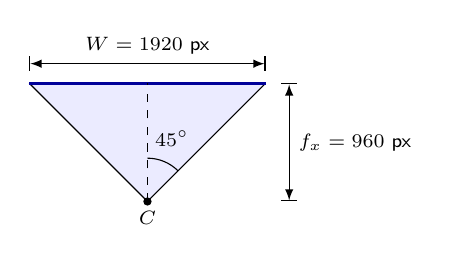
\begin{tikzpicture}[font=\sffamily\scriptsize, >=latex]
        \fill[blue!8] (0,0) -- (-1.5,1.5) -- (1.5,1.5) -- cycle;
        \draw (0,0) -- (-1.5,1.5);
        \draw (0,0) -- (1.5,1.5);
        \draw[very thick, blue!60!black] (-1.5,1.5) -- (1.5,1.5);
        \draw[dashed] (0,0) -- (0,1.5);
        \draw (0,0.55) arc[start angle=90, end angle=45, radius=0.55];
        \node at (0.31,0.8) {$45^\circ$};
        \fill (0,0) circle (1.5pt) node[below] {$C$};
        \draw[|<->|] (-1.5,1.75) -- (1.5,1.75) node[midway, above] {$W=1920$ px};
        \draw[|<->|] (1.8,0) -- (1.8,1.5) node[midway, right] {$f_x=960$ px};
      \end{tikzpicture}\\[0.6em]
      \begin{minipage}{\linewidth}\scriptsize\raggedright
        \textbf{Worked example (top view):} a 1920-pixel-wide image with $\mathrm{HFOV}=90^\circ$ has
        \[ f_x=\frac{W/2}{\tan(\mathrm{HFOV}/2)}=\frac{960}{\tan45^\circ}=960\ \text{px}. \]
        The same camera from its hardware: a 3.0\,mm lens on pixels of pitch $3.125\,\mu\mathrm{m}$ gives $f_x=3.0\,\mathrm{mm}/3.125\,\mu\mathrm{m}=960$ px, and the 1920 pixels span 6.0\,mm.
      \end{minipage}
  \end{columns}
\end{frame}

\begin{frame}{Extrinsics and the Projection Matrix}
  \begin{columns}[T,onlytextwidth]
    \column{0.55\textwidth}
      \begin{itemize}\footnotesize\itemsep0.3em
        \item \textbf{Extrinsics $[R\mid\mathbf{t}]$:} a rigid motion takes world coordinates to camera coordinates,
        \[ \mathbf{X}_c = R\,\mathbf{X}_w+\mathbf{t}. \]
        $R\in SO(3)$, the group of 3D rotations ($R^\top R=I$, $\det R=1$), has 3 degrees of freedom (DoF); $\mathbf{t}\in\mathbb{R}^3$ has 3 more.
        \item In homogeneous form, $\tilde{\mathbf{X}}_c=T\,\tilde{\mathbf{X}}_w$ with $T=\begin{bmatrix}R&\mathbf{t}\\ \mathbf{0}^\top&1\end{bmatrix}\in SE(3)$, the group of rigid motions.
        \item \textbf{Camera centre:} $\mathbf{X}_c=\mathbf{0}$ gives $\mathbf{C}=-R^\top\mathbf{t}$ in world coordinates; $\mathbf{t}$ is the world origin expressed in camera coordinates.
        \item \textbf{Projection:}
        \[ \lambda\,\tilde{\mathbf{x}} = K\,[R\mid\mathbf{t}]\,\tilde{\mathbf{X}} = P\,\tilde{\mathbf{X}}. \]
        $P$ is $3\times4$ and defined up to scale: $12-1=11$ DoF, 5 intrinsic plus 6 extrinsic. $\lambda=Z_c$ is the depth; $\pi(K,R,\mathbf{t},\mathbf{X})$ denotes the resulting pixel $\mathbf{x}$.
      \end{itemize}
    \column{0.43\textwidth}
      \vspace{0.6em}
      \begin{tcolorbox}[colframe=KAred, colback=gray!6, boxrule=0.5pt, left=4pt, right=4pt, top=3pt, bottom=3pt]
        \footnotesize
        \textbf{Worked example}\\[0.3em]
        $f_x=f_y=500$, $s=0$, $(c_x,c_y)=(320,240)$; $R=I$, $\mathbf{t}=(0,0,4)^\top$; world point $\mathbf{X}_w=(1,\,0.5,\,0)^\top$, in metres.
        \begin{enumerate}\itemsep0.3em
          \item $\mathbf{X}_c=R\,\mathbf{X}_w+\mathbf{t}=(1,\,0.5,\,4)^\top$
          \item $K\mathbf{X}_c=(500\cdot1+320\cdot4,\;500\cdot0.5+240\cdot4,\;4)^\top$\\ $=(1780,\,1210,\,4)^\top$
          \item Divide by $\lambda=4$: $(u,v)=(445,\,302.5)$
          \item $\mathbf{C}=-R^\top\mathbf{t}=(0,0,-4)^\top$: the camera is 4\,m behind the world origin.
        \end{enumerate}
      \end{tcolorbox}
  \end{columns}
\end{frame}

\begin{frame}{Back-Projection: A Pixel Is a Ray}
  \begin{columns}[T,onlytextwidth]
    \column{0.64\textwidth}
      \begin{itemize}\footnotesize\itemsep0.3em
        \item \textbf{Back-projection} inverts the projection for a pixel whose depth $Z$ is known ($s=0$):
        \[ \mathbf{X}_c = Z\,K^{-1}\tilde{\mathbf{x}} = \Big(Z\,\frac{u-c_x}{f_x},\;\; Z\,\frac{v-c_y}{f_y},\;\; Z\Big)^{\!\top}, \]
        and $\mathbf{X}_w = R^\top(\mathbf{X}_c-\mathbf{t})$ in world coordinates. Check: $(445,\,302.5)$ at $Z=4$ gives $(4\cdot125/500,\;4\cdot62.5/500,\;4)=(1,\,0.5,\,4)$.
        \item Without $Z$ a pixel fixes only a ray, $\{\mu\,K^{-1}\tilde{\mathbf{x}}:\mu>0\}$. Depth means the $Z$ coordinate, measured along the optical axis; the distance along an off-axis ray is larger.
        \item \textbf{Scale ambiguity:} scaling the scene and the translation by the same $\alpha>0$ changes no pixel, since $K[R\mid\alpha\mathbf{t}]\,(\alpha\mathbf{X}_w,1)^\top=\alpha\,K[R\mid\mathbf{t}]\,\tilde{\mathbf{X}}$. One moving camera therefore recovers depth only up to scale. A stereo pair with a known distance between the cameras (the baseline), an object of known size, or an IMU (inertial measurement unit: accelerometers and gyroscopes) fixes it.
        \item A depth map $D(\mathbf{p})$, one depth per pixel $\mathbf{p}$, back-projects to a \textbf{point cloud}: an unordered set of 3D points $\{D(\mathbf{p})\,K^{-1}\tilde{\mathbf{p}}\}$, often with each pixel's colour.
      \end{itemize}
    \column{0.34\textwidth}
      \centering
      \begin{tikzpicture}[font=\sffamily\scriptsize, >=latex, scale=0.86, every node/.style={transform shape}]
        \coordinate (C1) at (0,0);
        \coordinate (C2) at (1,0);
        \coordinate (C3) at (2,0);
        \coordinate (X) at (0.6,1.6);
        \coordinate (X2) at (1.2,3.2);
        \foreach \c in {0,1,2} {\draw[thick, black!55] (\c-0.3,0.4) -- (\c+0.3,0.4);}
        \draw[black!75] (C1) -- (X2);
        \draw[thick, blue!70!black] (C2) -- (X);
        \draw[thick, orange!85!black] (C3) -- (X2);
        \fill (C1) circle (1.5pt) node[below] {$C_1$};
        \fill[blue!70!black] (C2) circle (1.5pt) node[below] {$C_2$};
        \fill[orange!85!black] (C3) circle (1.5pt) node[below] {$C_2'$};
        \fill[blue!70!black] (X) circle (1.6pt) node[left] {$\mathbf{X}$};
        \fill[orange!85!black] (X2) circle (1.6pt) node[left] {$2\mathbf{X}$};
        \fill ($(C1)!0.25!(X)$) circle (1.2pt);
        \fill[blue!70!black] ($(C2)!0.25!(X)$) circle (1.2pt);
        \fill[orange!85!black] ($(C3)!0.125!(X2)$) circle (1.2pt);
        \draw[|<->|, blue!70!black] (0,-0.62) -- (1,-0.62) node[midway, below] {baseline $B$};
        \draw[|<->|, orange!85!black] (0,-1.2) -- (2,-1.2) node[midway, below] {$2B$};
      \end{tikzpicture}\\[0.4em]
      {\scriptsize Top view, short bars are image planes. Doubling the scene and the baseline (orange) gives the same pixels: the orange ray is parallel to the blue one, and the black ray is shared.\par}
  \end{columns}
\end{frame}

\begin{frame}{Lens Distortion}
  \begin{columns}[T,onlytextwidth]
    \column{0.60\textwidth}
      \begin{itemize}\footnotesize\itemsep0.25em
        \item \textbf{Lens distortion:} a real lens departs from the pinhole's central projection, mostly because its magnification changes with the distance from the principal point, so straight lines can image as curves. The pinhole model holds only after this is removed.
        \item On normalized coordinates $(x,y)=(X/Z,\,Y/Z)$, the pinhole image for $f=1$, with $r^2=x^2+y^2$:
        \[ \begin{aligned} x_d &= x\,(1+k_1r^2+k_2r^4+k_3r^6) + 2p_1xy + p_2(r^2+2x^2),\\ y_d &= y\,(1+k_1r^2+k_2r^4+k_3r^6) + p_1(r^2+2y^2) + 2p_2xy,\\ u &= f_x\,x_d+c_x,\quad v = f_y\,y_d+c_y\quad (s=0\text{ as in OpenCV}). \end{aligned} \]
        \item \textbf{Radial} terms $k_1,k_2,k_3$ move points along the radius, more towards the border: barrel distortion when $1+k_1r^2+k_2r^4+k_3r^6$ decreases with $r$ (usually $k_1<0$), pincushion when it increases.
        \item \textbf{Tangential} (decentering) terms $p_1,p_2$ come from lens elements that are not exactly centred and parallel to the sensor.
        \item \textbf{Calibration} estimates $K$ and these coefficients (next slides); images or keypoints are then undistorted by inverting this map numerically.
      \end{itemize}
    \column{0.38\textwidth}
      \centering
      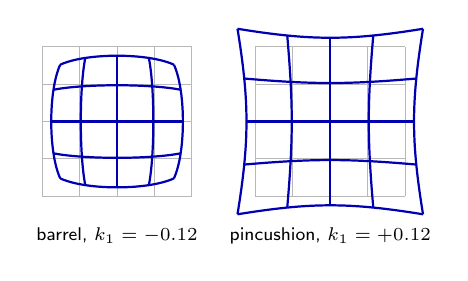
\begin{tikzpicture}[font=\sffamily\scriptsize, scale=0.95, every node/.style={transform shape}]
        \foreach \kk/\xo/\lab in {-0.12/0/{barrel, $k_1=-0.12$}, 0.12/2.85/{pincushion, $k_1=+0.12$}} {
          \begin{scope}[xshift=\xo cm]
            \foreach \g in {-1,-0.5,0,0.5,1} {
              \draw[black!28] (\g,-1) -- (\g,1);
              \draw[black!28] (-1,\g) -- (1,\g);
            }
            \foreach \g in {-1,-0.5,0,0.5,1} {
              \draw[blue!70!black, thick] plot[domain=-1:1, samples=25, smooth, variable=\t] ({(\g)*(1+(\kk)*((\g)*(\g)+(\t)*(\t)))}, {(\t)*(1+(\kk)*((\g)*(\g)+(\t)*(\t)))});
              \draw[blue!70!black, thick] plot[domain=-1:1, samples=25, smooth, variable=\t] ({(\t)*(1+(\kk)*((\g)*(\g)+(\t)*(\t)))}, {(\g)*(1+(\kk)*((\g)*(\g)+(\t)*(\t)))});
            }
            \node[below] at (0,-1.3) {\lab};
          \end{scope}
        }
      \end{tikzpicture}\\[0.4em]
      {\scriptsize Grey: a square grid of half-width 1 in normalized coordinates. Blue: its image under the radial term $k_1$ alone. A real camera with a 6\,mm lens, calibrated by Zhang (MSR-TR-98-71, Table~1), has $k_1=-0.228$, $k_2=0.190$: barrel.\par}\vspace{0.3em}
      {\scriptsize Model: Brown (1971), Eq.~20, written there as the inverse correction; forward form and names from OpenCV calib3d, \href{https://docs.opencv.org/4.x/d9/d0c/group__calib3d.html}{docs.opencv.org}.\par}
  \end{columns}
\end{frame}

\begin{frame}{Homographies: Planes and Pure Rotations}
  \begin{columns}[T,onlytextwidth]
    \column{0.60\textwidth}
      \begin{itemize}\scriptsize\itemsep0.15em
        \item A \textbf{homography} is an invertible $3\times3$ matrix on homogeneous pixels, $\tilde{\mathbf{x}}'\sim H\tilde{\mathbf{x}}$, defined up to scale (8~DoF). It maps lines to lines.
        \item \textbf{Plane-induced homography:} put the world plane at $Z=0$. The third column $\mathbf{r}_3$ of $R=[\mathbf{r}_1\ \mathbf{r}_2\ \mathbf{r}_3]$ then drops out:
        \[ \lambda\tilde{\mathbf{x}} = K[\mathbf{r}_1\ \mathbf{r}_2\ \mathbf{r}_3\ \mathbf{t}]\,(X,Y,0,1)^\top = \underbrace{K[\mathbf{r}_1\ \mathbf{r}_2\ \mathbf{t}]}_{H}\,(X,Y,1)^\top. \]
        Two views of the same plane are therefore related by $H_2H_1^{-1}$.
        \item \textbf{Pure rotation} (no translation, as for a panorama): $\tilde{\mathbf{x}}'\sim KRK^{-1}\tilde{\mathbf{x}}$ for every point, whatever its depth.
        \item \textbf{DLT} (direct linear transform): with $\mathbf{a}^\top,\mathbf{b}^\top,\mathbf{c}^\top$ the rows of $H$, $u'=\mathbf{a}^\top\tilde{\mathbf{x}}/\mathbf{c}^\top\tilde{\mathbf{x}}$ and $v'=\mathbf{b}^\top\tilde{\mathbf{x}}/\mathbf{c}^\top\tilde{\mathbf{x}}$ give two equations per match,
        \[ \mathbf{a}^\top\tilde{\mathbf{x}}-u'\,\mathbf{c}^\top\tilde{\mathbf{x}}=0,\qquad \mathbf{b}^\top\tilde{\mathbf{x}}-v'\,\mathbf{c}^\top\tilde{\mathbf{x}}=0, \]
        linear in the 9 entries $\mathbf{h}$ of $H$. Stack $n\geq4$ matches into $A\mathbf{h}=\mathbf{0}$ ($A$ is $2n\times9$); $\mathbf{h}$ is the right singular vector of $A$ with the smallest singular value (SVD). First translate and scale each image's points to zero mean and mean distance $\sqrt{2}$ (matrices $T$, $T'$), solve for $\hat{H}$, then undo it: $H=T'^{-1}\hat{H}\,T$.
        \item Wrong matches (outliers) ruin this fit; RANSAC (random sample consensus) removes them.
      \end{itemize}
    \column{0.38\textwidth}
      \centering
      \vspace{0.8em}
      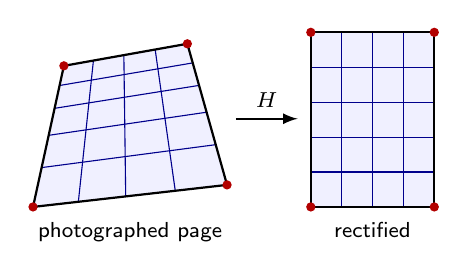
\begin{tikzpicture}[font=\sffamily\scriptsize, >=latex, scale=1.12, every node/.style={transform shape}, gridln/.style={blue!55!black, thin}]
        \fill[blue!6] (0,0) -- (2.2,0.25) -- (1.75,1.85) -- (0.35,1.6) -- cycle;
        \draw[gridln] (0.514,0.058) -- (0.685,1.660);
        \draw[gridln] (1.051,0.119) -- (1.030,1.721);
        \draw[gridln] (1.613,0.183) -- (1.385,1.785);
        \draw[gridln] (0.097,0.446) -- (2.072,0.706);
        \draw[gridln] (0.178,0.812) -- (1.968,1.074);
        \draw[gridln] (0.244,1.118) -- (1.883,1.378);
        \draw[gridln] (0.301,1.377) -- (1.811,1.633);
        \draw[thick] (0,0) -- (2.2,0.25) -- (1.75,1.85) -- (0.35,1.6) -- cycle;
        \foreach \p in {(0,0),(2.2,0.25),(1.75,1.85),(0.35,1.6)} {\fill[red!70!black] \p circle (1.5pt);}
        \node[below] at (1.1,-0.05) {photographed page};
        \begin{scope}[xshift=3.15cm]
          \fill[blue!6] (0,0) rectangle (1.4,1.98);
          \foreach \x in {0.35,0.7,1.05} {\draw[gridln] (\x,0) -- (\x,1.98);}
          \foreach \y in {0.396,0.792,1.188,1.584} {\draw[gridln] (0,\y) -- (1.4,\y);}
          \draw[thick] (0,0) rectangle (1.4,1.98);
          \foreach \p in {(0,0),(1.4,0),(1.4,1.98),(0,1.98)} {\fill[red!70!black] \p circle (1.5pt);}
          \node[below] at (0.7,-0.05) {rectified};
        \end{scope}
        \draw[->, thick] (2.3,1.0) -- (3.0,1.0) node[midway, above] {$H$};
      \end{tikzpicture}\\[0.5em]
      {\scriptsize Four corner matches (red) fix $H$, and every grid line of the photographed page lands on its place in the upright page. A bird's-eye view of a road applies the same mapping to the road plane. After Hartley and Zisserman (2004), Ch.~4 and~13.\par}
  \end{columns}
\end{frame}

\begin{frame}{Calibrating a Camera with a Planar Pattern}
  \begin{columns}[T,onlytextwidth]
    \column{0.61\textwidth}
      \begin{itemize}\scriptsize\itemsep0.25em
        \item Zhang's calibration method uses a flat pattern of known geometry, such as a printed checkerboard, as the plane $Z=0$, so every corner has known coordinates $(X,Y,0)$.
        \item The camera sees the pattern ``at a few (at least two) different orientations''; the camera or the board may move, and the motion need not be known.
        \item \textbf{Per view $i$:} detect the corners and fit the plane-induced $H_i=[\mathbf{h}_1\ \mathbf{h}_2\ \mathbf{h}_3]\sim K[\mathbf{r}_1\ \mathbf{r}_2\ \mathbf{t}]$ by DLT ($\mathbf{r}_1,\mathbf{r}_2,\mathbf{t}$ of view $i$, index dropped). Since $\mathbf{r}_1\perp\mathbf{r}_2$ and $\lVert\mathbf{r}_1\rVert=\lVert\mathbf{r}_2\rVert$,
        \[ \mathbf{h}_1^\top\omega\,\mathbf{h}_2=0,\qquad \mathbf{h}_1^\top\omega\,\mathbf{h}_1=\mathbf{h}_2^\top\omega\,\mathbf{h}_2,\qquad \omega=K^{-\top}K^{-1}. \]
        \item \textbf{Closed form:} two linear equations per view in the 6 entries of the symmetric $\omega$, solved by SVD; 3 views suffice in general, 2 with zero skew. Then $K$ follows from $\omega$, and $R_i,\mathbf{t}_i$ from each $H_i$.
        \item \textbf{Refinement:} nonlinear least squares over $K$, the distortion coefficients $\mathbf{k}$ and all poses, minimizing the squared \textbf{reprojection error}, the pixel distance between each observed corner $\mathbf{x}_{ij}$ and the projection of its known point $\mathbf{X}_j$, with the distortion map (coefficients $\mathbf{k}$) applied before $K$:
        \[ \textstyle\sum_i\sum_j \big\lVert\mathbf{x}_{ij}-\pi(K,\mathbf{k},R_i,\mathbf{t}_i,\mathbf{X}_j)\big\rVert^2. \]
        On Zhang's $640\times480$ camera with 5 views, the root-mean-square (RMS) error fell from 0.881\,px (closed form) to 0.335\,px.
      \end{itemize}
    \column{0.37\textwidth}
      \centering
      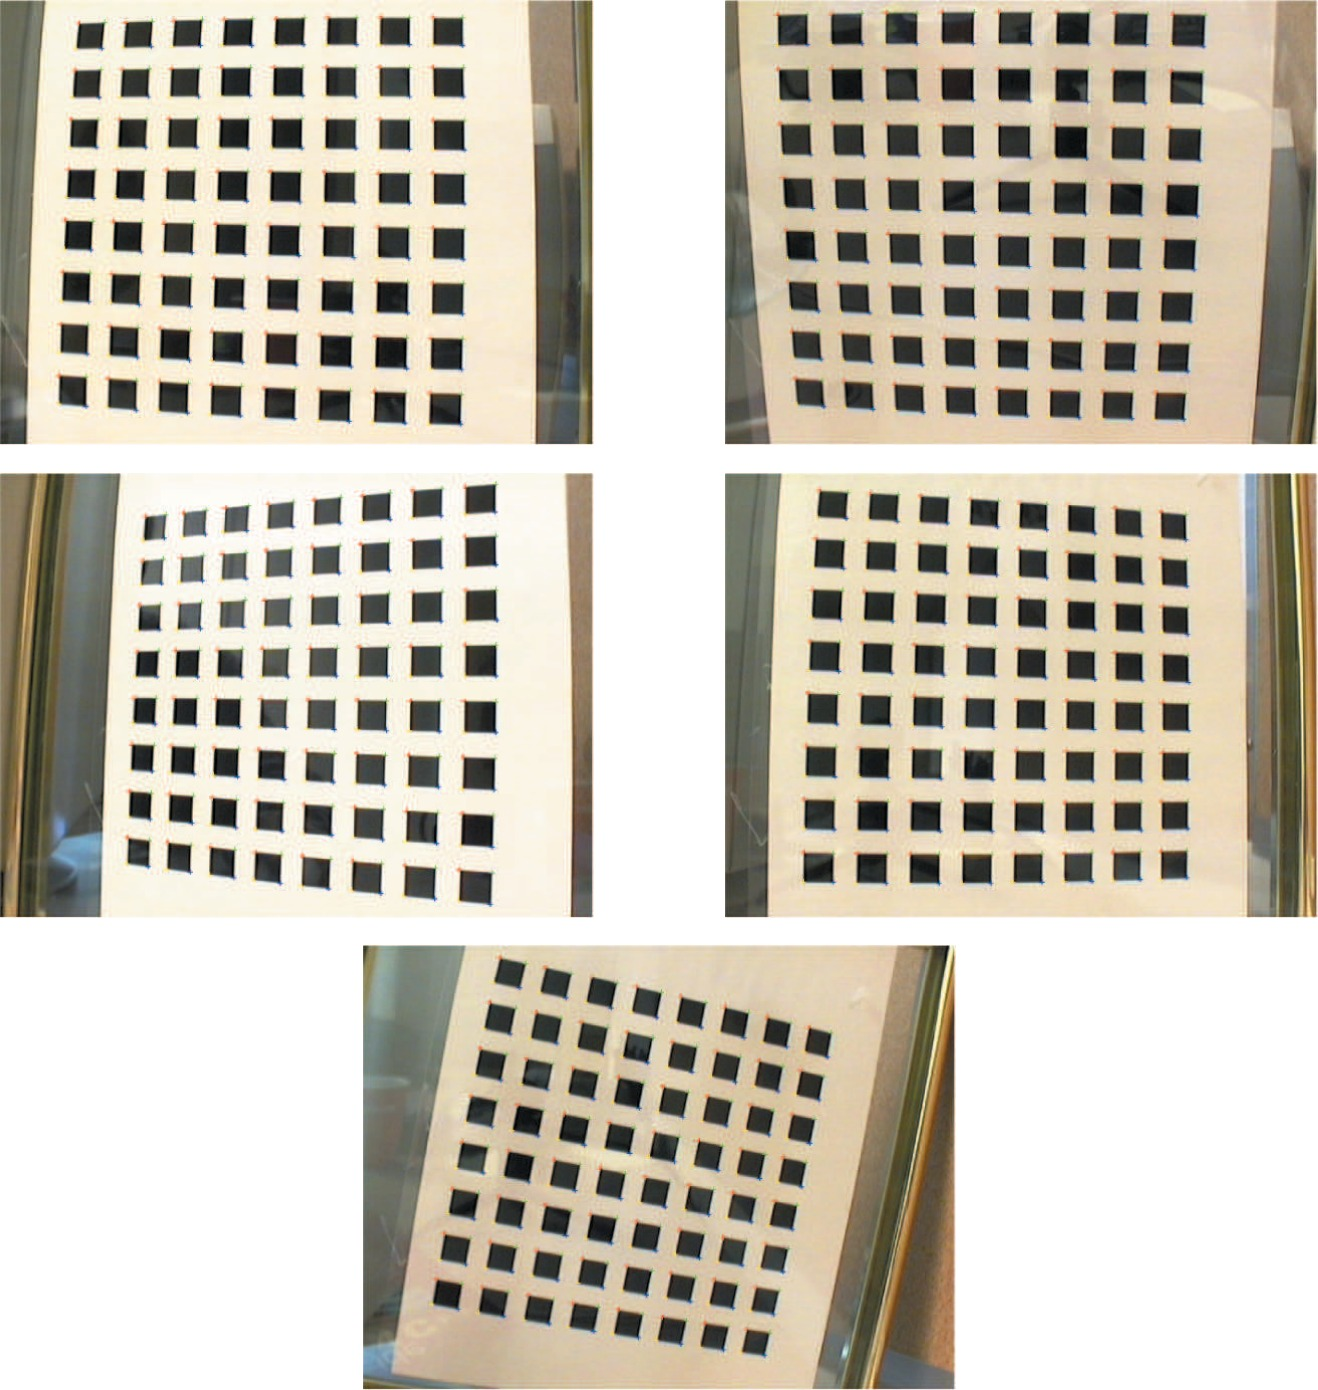
\includegraphics[width=\linewidth,height=0.53\textheight,keepaspectratio]{images/3d-vision/zhang_fig4_calibration_views.jpg}\\[0.2em]
      {\scriptsize The five views of Zhang's real-data experiment: $8\times8$ separate squares, 256 corners, 17\,cm wide. Z.~Zhang, ``A Flexible New Technique for Camera Calibration,'' IEEE TPAMI 2000, \href{https://doi.org/10.1109/34.888718}{doi:10.1109/34.888718}; figure from the report \href{https://www.microsoft.com/en-us/research/wp-content/uploads/2016/02/tr98-71.pdf}{MSR-TR-98-71}, Figure~4.\par}
  \end{columns}
\end{frame}
